\documentclass[12pt]{article}

\usepackage{fontspec}
\newfontfamily\handwriting{a-casual-handwritten-pen}[Path=../assets/fonts/,Extension=.ttf,Scale=1.5]
\newfontfamily\comic{Comic Neue}

\usepackage[utf8]{inputenc}
\usepackage{amsmath}
\usepackage{amssymb}
\usepackage{enumitem}
\usepackage{xcolor}
\usepackage{soul}
\usepackage{tikz}
\usepackage[most]{tcolorbox}
\usepackage{titlesec}
\usepackage{multicol}
\usepackage{environ}

\usetikzlibrary{fit, positioning, arrows.meta, decorations.pathreplacing}

% --- Custom Colors ---
\definecolor{primaryblue}{RGB}{42, 111, 151}
\definecolor{exbg}{RGB}{255, 240, 245}
\definecolor{rulebg}{RGB}{232, 245, 233}
\definecolor{highlight}{RGB}{255, 243, 176}
\definecolor{pinkanno}{RGB}{255, 105, 180}
\definecolor{purpleanno}{RGB}{147, 112, 219}
\definecolor{solutionbg}{RGB}{245, 245, 255}

% --- Header Styling ---
\titleformat{\section}{\color{primaryblue}\normalfont\Large\bfseries}{\thesection}{1em}{}
\titleformat{\subsection}{\color{primaryblue}\normalfont\large\bfseries}{\thesubsection}{1em}{}

% --- Friendly Boxes ---
% --- Auto-numbered Example Box ---
\newcounter{examplenum}

\newtcolorbox{friendlyexbox}[1]{
    colback=exbg,
    colframe=pinkanno!50,
    arc=5pt,
    title=\textbf{#1},
    coltitle=black,
    attach title to upper,
    after title={:\quad}
}

\newenvironment{friendlyex}{%
    \refstepcounter{examplenum}%
    \begin{friendlyexbox}{Example \theexamplenum}%
}{%
    \end{friendlyexbox}%
}

\newtcolorbox{friendlyrule}[1]{
    colback=rulebg,
    colframe=primaryblue!30,
    arc=5pt,
    fonttitle=\bfseries,
    title={#1},
    coltitle=primaryblue
}

\newcommand{\funhl}[1]{\sethlcolor{highlight}\hl{#1}}

% --- Show/Hide Solutions ---
\newif\ifshowsolutions

% Uncomment the next line to show solutions.
\showsolutionstrue

\newsavebox{\solutionmeasurebox}

\NewEnviron{solutionbox}{
\ifshowsolutions
\begin{tcolorbox}[
    colback=solutionbg,
    colframe=purpleanno!45,
    arc=5pt,
    title={Solution},
    coltitle=primaryblue,
    fonttitle=\bfseries
]
\BODY
\end{tcolorbox}
\else
\sbox{\solutionmeasurebox}{\begin{minipage}{\dimexpr\linewidth-10pt\relax}\BODY\end{minipage}}
\vspace{\dimexpr\ht\solutionmeasurebox+\dp\solutionmeasurebox+3em\relax}
\fi
}

\begin{document}
\handwriting

\begin{center}
    \Large\textbf{\color{primaryblue}Module 2 Lesson 3\\Quadratic Functions and Applications} \\
    \vspace{0.2cm}
    \hrule
\end{center}

\section*{Objectives}

\begin{friendlyrule}{In this lesson, we will learn how to}
\begin{itemize}
    \item identify the vertex and axis of symmetry of a parabola;
    \item find the vertex using a formula and using vertex form;
    \item sketch a parabola from the sign of $a$, $h$, and $k$;
    \item solve maximum/minimum application problems.
\end{itemize}
\end{friendlyrule}

\section*{1. Parabolas}

The graph of a quadratic function, $f(x)=ax^2+bx+c$, is a U-shaped curve called a \funhl{parabola}.

\begin{center}
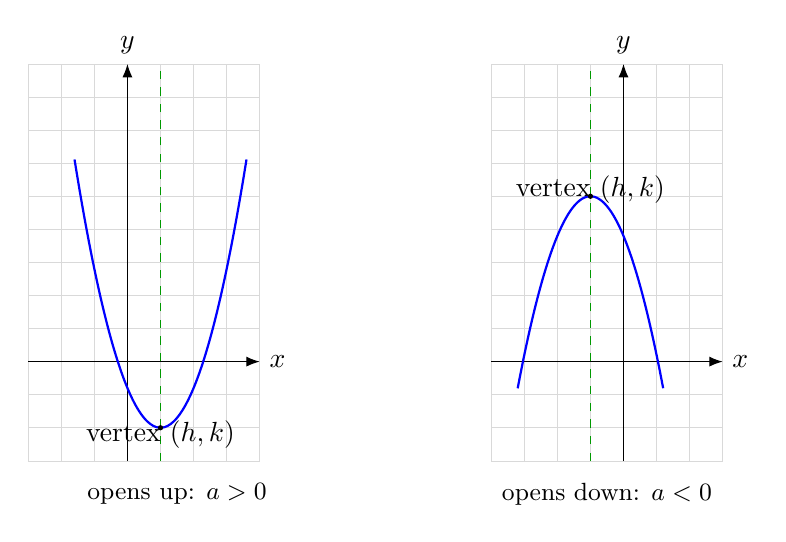
\begin{tikzpicture}[scale=0.42]
% Left: opens up
\begin{scope}
\draw[step=1, gray!30, very thin] (-3,-3) grid (4,9);
\draw[-{Latex}] (-3,0) -- (4,0) node[right] {$x$};
\draw[-{Latex}] (0,-3) -- (0,9) node[above] {$y$};
\draw[green!60!black, dashed] (1,-3) -- (1,9);
\draw[blue, thick, domain=-1.6:3.6, samples=60, smooth] plot (\x, {1.2*(\x-1)*(\x-1) - 2});
\fill[black] (1,-2) circle (0.08);
\node[below] at (1,-1.5) {vertex $(h,k)$};
\node at (1.5,-4) {\small opens up: $a>0$};
\end{scope}
% Right: opens down
\begin{scope}[shift={(15,0)}]
\draw[step=1, gray!30, very thin] (-4,-3) grid (3,9);
\draw[-{Latex}] (-4,0) -- (3,0) node[right] {$x$};
\draw[-{Latex}] (0,-3) -- (0,9) node[above] {$y$};
\draw[green!60!black, dashed] (-1,-3) -- (-1,9);
\draw[blue, thick, domain=-3.2:1.2, samples=60, smooth] plot (\x, {-1.2*(\x+1)*(\x+1) + 5});
\fill[black] (-1,5) circle (0.08);
\node[above] at (-1,4.5) {vertex $(h,k)$};
\node at (-0.5,-4) {\small opens down: $a<0$};
\end{scope}
\end{tikzpicture}
\end{center}

\begin{friendlyrule}{Vertex and Axis of Symmetry}
\begin{itemize}
    \item \funhl{Vertex}: the turning point of the parabola.
    \item If $a>0$, the parabola opens upward and the vertex is the \textbf{minimum} point.
    \item If $a<0$, the parabola opens downward and the vertex is the \textbf{maximum} point.
    \item \funhl{Axis of symmetry}: the vertical line through the vertex; the graph is a mirror image across this line.
\end{itemize}
\end{friendlyrule}

\section*{2. Finding the Vertex by Formula}

\begin{friendlyrule}{Vertex Formula}
For $f(x)=ax^2+bx+c$, the vertex $(h,k)$ is given by

\[
h=\frac{-b}{2a},\qquad k=f(h).
\]

The axis of symmetry is $x=h$.
\end{friendlyrule}

\begin{friendlyex}{}
Find the vertex and axis of symmetry of the functions
\begin{itemize}
    \item[(a)] $f(x)=3x^2+6x+5$
    \item[(b)] $f(x)=-2x^2+12x+15$
\end{itemize}
\end{friendlyex}

 

\begin{solutionbox}
\textbf{(a)} $a=3$, $b=6$:

\[
h=\frac{-6}{2(3)}=-1,\qquad k=f(-1)=3(1)-6+5=2.
\]

Vertex: $(-1,2)$. Axis of symmetry: $x=-1$.

\textbf{(b)} $a=-2$, $b=12$:

\[
h=\frac{-12}{2(-2)}=3,\qquad k=f(3)=-2(9)+36+15=33.
\]

Vertex: $(3,33)$. Axis of symmetry: $x=3$.
\end{solutionbox}

  

\section*{3. Vertex Form}

\begin{friendlyrule}{Vertex Form}
\[
f(x)=a(x-h)^2+k.
\]
\begin{itemize}
    \item The vertex is $(h,k)$.
    \item The axis of symmetry is $x=h$.
    \item If $a>0$ the graph opens up; if $a<0$ the graph opens down.
\end{itemize}
\end{friendlyrule}

\begin{friendlyex}{}
Find the vertex, axis of symmetry, and direction of the parabola formed by each function.
\begin{itemize}
    \item[(a)] $f(x)=-4(x-3)^2+5$
    \item[(b)] $f(x)=x^2+10x+22$
\end{itemize}
\end{friendlyex}

 

\begin{solutionbox}
\textbf{(a)} Already in vertex form with $a=-4$, $h=3$, $k=5$. Vertex: $(3,5)$. Axis: $x=3$. Since $a=-4<0$, the parabola opens \textbf{down}.

\textbf{(b)} Complete the square:

\[
x^2+10x+22=(x^2+10x+25)-25+22=(x+5)^2-3.
\]

So $h=-5$, $k=-3$. Vertex: $(-5,-3)$. Axis: $x=-5$. Since $a=1>0$, the parabola opens \textbf{up}.
\end{solutionbox}

  

\section*{4. Sketching a Parabola from $a$, $h$, $k$}

\begin{friendlyex}{}
Given a quadratic function defined by $f(x)=a(x-h)^2+k$, determine what the graph would look like based on the given criteria (sketch on the blank axes provided).
\begin{itemize}
    \item[1.] $a>0$, $h<0$, $k<0$
    \item[2.] $a<0$, $h>0$, $k<0$
    \item[3.] $a<0$, $h<0$, $k>0$
\end{itemize}
\end{friendlyex}

\begin{center}
\begin{tikzpicture}[scale=0.5]
\foreach \i in {0,1,2}{
\begin{scope}[shift={(10*\i,0)}]
\draw[-{Latex}] (-4,0) -- (4,0);
\draw[-{Latex}] (0,-4) -- (0,4);
\end{scope}
}
\end{tikzpicture}
\end{center}

 

\begin{solutionbox}
\textbf{1.} $a>0$ (opens up), vertex $(h,k)$ with $h<0,\,k<0$ (vertex in Quadrant III). Since the vertex is below the $x$-axis and the parabola opens up, it crosses the $x$-axis twice.

\textbf{2.} $a<0$ (opens down), vertex with $h>0,\,k<0$ (vertex in Quadrant IV). Since the vertex is already below the $x$-axis and the parabola opens further down, it \textbf{never} crosses the $x$-axis.

\textbf{3.} $a<0$ (opens down), vertex with $h<0,\,k>0$ (vertex in Quadrant II). Since the vertex is above the $x$-axis and the parabola opens down, it crosses the $x$-axis twice.

\begin{center}
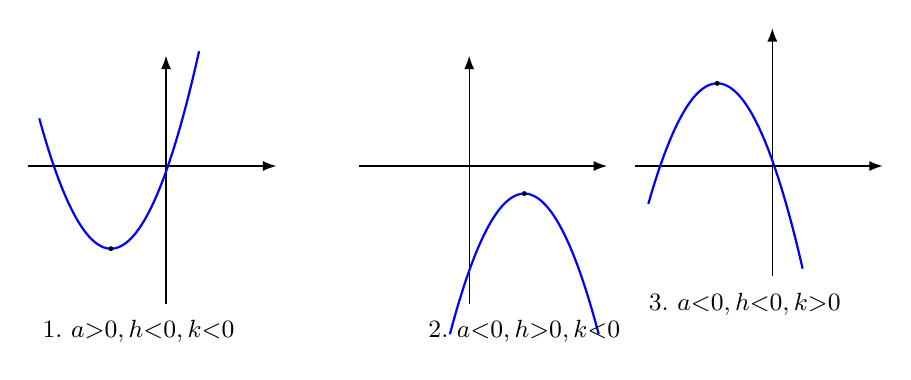
\begin{tikzpicture}[scale=0.35]
% Case 1: a>0, h<0,k<0
\begin{scope}
\draw[-{Latex}] (-5,0) -- (4,0);
\draw[-{Latex}] (0,-5) -- (0,4);
\draw[blue, thick, domain=-4.6:1.2, samples=50, smooth] plot (\x, {0.7*(\x+2)*(\x+2)-3});
\fill (-2,-3) circle (0.09);
\node at (-1,-6) {\small $1.\ a{>}0,h{<}0,k{<}0$};
\end{scope}
% Case 2: a<0, h>0, k<0
\begin{scope}[shift={(11,0)}]
\draw[-{Latex}] (-4,0) -- (5,0);
\draw[-{Latex}] (0,-5) -- (0,4);
\draw[blue, thick, domain=-0.7:4.7, samples=50, smooth] plot (\x, {-0.7*(\x-2)*(\x-2)-1});
\fill (2,-1) circle (0.09);
\node at (2,-6) {\small $2.\ a{<}0,h{>}0,k{<}0$};
\end{scope}
% Case 3: a<0, h<0, k>0
\begin{scope}[shift={(22,0)}]
\draw[-{Latex}] (-5,0) -- (4,0);
\draw[-{Latex}] (0,-4) -- (0,5);
\draw[blue, thick, domain=-4.5:1.1, samples=50, smooth] plot (\x, {-0.7*(\x+2)*(\x+2)+3});
\fill (-2,3) circle (0.09);
\node at (-1,-5) {\small $3.\ a{<}0,h{<}0,k{>}0$};
\end{scope}
\end{tikzpicture}
\end{center}
\end{solutionbox}

  

\section*{5. Applications: Maximum and Minimum}

\begin{friendlyrule}{Maximum or Minimum Value}
\begin{itemize}
    \item If the graph opens up, the $k$-value of the vertex is a \textbf{minimum} value.
    \item If the graph opens down, the $k$-value of the vertex is a \textbf{maximum} value.
\end{itemize}
\end{friendlyrule}

\begin{friendlyex}{}
\textbf{Height of a Missile.} A missile is launched with an initial velocity of $150$ ft/sec from a height of $40$ ft. The function

\[
H(t)=-5t^2+150t+40
\]

gives the height of the missile $t$ seconds after launch. Determine the time at which the missile reaches its maximum height, and find that maximum height.
\end{friendlyex}

 

\begin{solutionbox}
Here $a=-5$, $b=150$:

\[
h=\frac{-150}{2(-5)}=15.
\]

\[
H(15)=-5(15)^2+150(15)+40=-1125+2250+40=1165.
\]

The missile reaches its maximum height of $1165$ feet at $t=15$ seconds.
\end{solutionbox}

  

\begin{friendlyex}{}
\textbf{Minimizing Cost.} A company's total cost $C(q)$ in dollars for producing $q$ units is modeled by

\[
C(q)=2q^2-160q+5000.
\]

Determine the production level at which the cost is minimum, and compute the minimum cost.
\end{friendlyex}

 

\begin{solutionbox}
Here $a=2$, $b=-160$:

\[
h=\frac{-(-160)}{2(2)}=\frac{160}{4}=40.
\]

\[
C(40)=2(40)^2-160(40)+5000=3200-6400+5000=1800.
\]

The minimum cost is $\$1800$, achieved at a production level of $40$ units.
\end{solutionbox}

  

\begin{friendlyex}{}
\textbf{Maximizing Area.} A farmer has $200$ ft of fencing and wants to build three identical adjacent rectangular corrals, as pictured (each corral has depth $x$; the three together span a total width $y$). Determine the dimensions that maximize the total area, and find the area of each individual corral.
\end{friendlyex}

\begin{center}
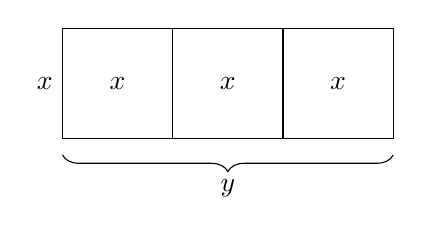
\begin{tikzpicture}[scale=0.7]
\draw (0,0) rectangle (6,2);
\draw (2,0) -- (2,2);
\draw (4,0) -- (4,2);
\node[left] at (0,1) {$x$};
\node at (1,1) {$x$};
\node at (3,1) {$x$};
\node at (5,1) {$x$};
\draw[decorate, decoration={brace, amplitude=6pt, mirror}] (0,-0.3) -- (6,-0.3);
\node at (3,-0.9) {$y$};
\end{tikzpicture}
\end{center}

 

\begin{solutionbox}
There are $4$ vertical fence segments (each of length $x$) and $2$ horizontal segments (top and bottom, each of length $y$):

\[
4x+2y=200\ \Longrightarrow\ y=100-2x.
\]

The total area is

\[
A(x)=xy=x(100-2x)=100x-2x^2.
\]

This is a downward parabola in $x$, with $a=-2$, $b=100$:

\[
x=\frac{-100}{2(-2)}=25.
\]

Then $y=100-2(25)=50$.

Maximum total area:

\[
A(25)=25(50)=1250\text{ sq ft.}
\]

Each individual corral has area

\[
\frac{1250}{3}\approx 416.7\text{ sq ft.}
\]
\end{solutionbox}

  

\section*{Summary}

\begin{friendlyrule}{Key Ideas}
\begin{itemize}
    \item The graph of $f(x)=ax^2+bx+c$ is a parabola with vertex $\left(\dfrac{-b}{2a}, f\left(\dfrac{-b}{2a}\right)\right)$.
    \item In vertex form $f(x)=a(x-h)^2+k$, the vertex is $(h,k)$ directly.
    \item If $a>0$ the parabola opens up (vertex is a minimum); if $a<0$ it opens down (vertex is a maximum).
    \item Many real-world optimization problems (maximizing area, minimizing cost, finding maximum height) reduce to finding the vertex of a quadratic function.
\end{itemize}
\end{friendlyrule}

\end{document}
